\usepackage[a4paper,left=17mm,right=17mm,top=26mm,bottom=21mm,headheight=20pt,headsep=10mm]{geometry}
\usepackage{fix-cm}
\usepackage{fontspec}
\setmainfont{texgyreheros-regular.otf}[BoldFont=texgyreheros-bold.otf,ItalicFont=texgyreheros-italic.otf]
\setmonofont{lmmono10-regular.otf}
\usepackage[table]{xcolor}
\usepackage{array,booktabs,ragged2e}
\newcolumntype{L}[1]{>{\raggedright\arraybackslash}p{\dimexpr #1\linewidth-2\tabcolsep\relax}}
\usepackage{amsmath}
\usepackage{tikz}
\usetikzlibrary{arrows.meta,positioning}
\usepackage{fancyhdr,lastpage}
\usepackage{fancyvrb}
\usepackage{titlesec}
\usepackage{hyperref}
\definecolor{Navy}{HTML}{112744}
\definecolor{Blue}{HTML}{2463AD}
\definecolor{Ink}{HTML}{23354C}
\definecolor{Muted}{HTML}{586A80}
\definecolor{Pale}{HTML}{EDF4FC}
\definecolor{Stripe}{HTML}{F5F8FC}
\definecolor{Border}{HTML}{DCE5EF}
\definecolor{Amber}{HTML}{FFF5E4}
\hypersetup{colorlinks=true,urlcolor=Blue,linkcolor=Blue,pdftitle={BizWizard - \DocumentTitle},pdfauthor={BizWizard project}}
\pagestyle{fancy}
\fancyhf{}
\fancyhead[L]{\textcolor{Blue}{\bfseries BW}\quad\textcolor{Navy}{\bfseries BizWizard}}
\fancyhead[R]{\footnotesize\textcolor{Muted}{\DocumentTitle\ | Topic E}}
\fancyfoot[L]{\scriptsize\textcolor{Muted}{BizWizard | \DocumentTitle}}
\fancyfoot[R]{\scriptsize\textcolor{Muted}{\thepage\ / \pageref*{LastPage}}}
\renewcommand{\headrulewidth}{0pt}
\renewcommand{\footrulewidth}{0.3pt}
\renewcommand{\footrule}{\hbox to\headwidth{\color{Border}\leaders\hrule height \footrulewidth\hfill}}
\setlength{\parindent}{0pt}
\setlength{\parskip}{6pt}
\setlength{\emergencystretch}{2em}
\raggedbottom
\AtBeginDocument{\fontsize{10}{14}\selectfont\color{Ink}\raggedright}
\titleformat{\subsection}{\color{Navy}\bfseries\fontsize{12}{16}\selectfont}{}{0pt}{}
\titlespacing*{\subsection}{0pt}{9pt}{4pt}
\newcommand{\DocSection}[3]{%
  {\color{Blue}\bfseries\fontsize{9}{12}\selectfont #1\par}\vspace{5pt}%
  {\color{Navy}\bfseries\fontsize{24}{28}\selectfont #2\par}\vspace{3pt}%
  {\color{Muted}\fontsize{10.5}{15}\selectfont #3\par}\vspace{6pt}}
\newcommand{\SmallText}[1]{{\color{Muted}\fontsize{8.5}{11.5}\selectfont #1\par}}
\newcommand{\EvidenceFile}[1]{\href{https://github.com/mahfuz-saim/bizwizard/blob/main/evidence/submission/#1}{\nolinkurl{#1}}}
\newcommand{\EvidenceRevision}{\SmallText{Recorded on 18 October 2026 (UTC), from clean revision \texttt{8f394d2d074b}. These are saved results, not a fresh test of the current release. Each JSON report includes the full revision and source hashes.}}
\newcommand{\DocNote}[2][Pale]{%
  \par\begingroup\setlength{\fboxsep}{9pt}%
  \colorbox{#1}{\parbox{\dimexpr\linewidth-18pt\relax}{\raggedright #2}}\endgroup\par}
\newenvironment{ReportTable}[1]{%
  \par\begingroup\fontsize{9.2}{12.5}\selectfont%
  \setlength{\tabcolsep}{6pt}\setlength{\extrarowheight}{4pt}%
  \renewcommand{\arraystretch}{1.12}%
  \rowcolors{2}{white}{Stripe}\begin{tabular}{#1}}
  {\end{tabular}\endgroup\par}
\DefineVerbatimEnvironment{CodeBlock}{Verbatim}{fontsize=\footnotesize,frame=single,framerule=0.4pt,framesep=8pt,rulecolor=\color{Border},xleftmargin=0pt,xrightmargin=0pt}
\tikzset{docbox/.style={draw=Border,fill=Pale,rounded corners=4pt,align=left,inner sep=8pt,text width=0.265\linewidth,font=\fontsize{8.5}{11.5}\selectfont},flow/.style={-{Stealth[length=4pt]},draw=Blue,line width=0.8pt}}
\newcommand{\ArchitectureDiagram}{%
\begin{center}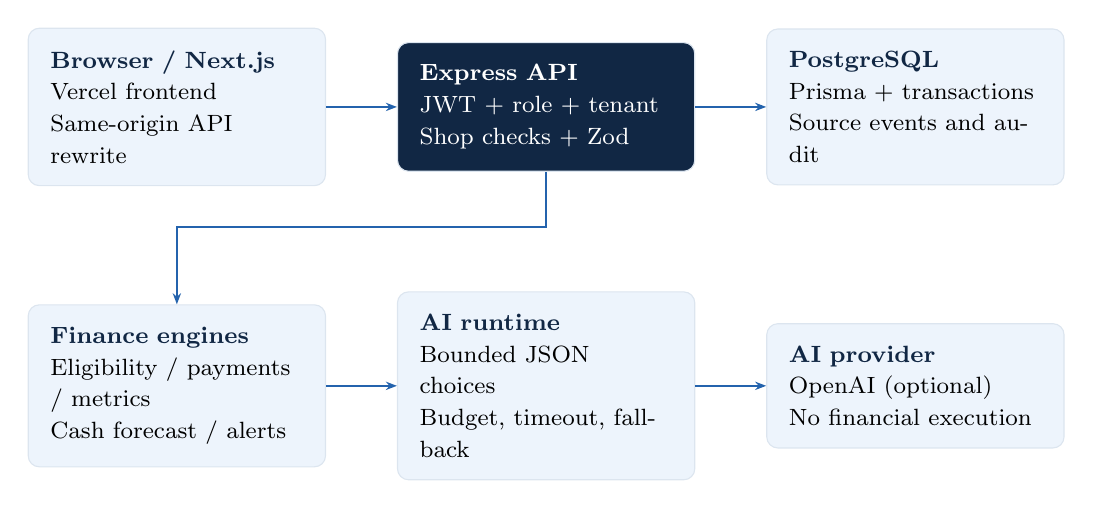
\begin{tikzpicture}[node distance=15mm and 9mm]
  \node[docbox] (browser) {\textcolor{Navy}{\bfseries Browser / Next.js}\\Vercel frontend\\Same-origin API rewrite};
  \node[docbox,right=of browser,fill=Navy,text=white] (api) {\bfseries Express API\normalfont\\JWT + role + tenant\\Shop checks + Zod};
  \node[docbox,right=of api] (db) {\textcolor{Navy}{\bfseries PostgreSQL}\\Prisma + transactions\\Source events and audit};
  \node[docbox,below=of browser] (rules) {\textcolor{Navy}{\bfseries Finance engines}\\Eligibility / payments / metrics\\Cash forecast / alerts};
  \node[docbox,right=of rules] (ai) {\textcolor{Navy}{\bfseries AI runtime}\\Bounded JSON choices\\Budget, timeout, fallback};
  \node[docbox,right=of ai] (external) {\textcolor{Navy}{\bfseries AI provider}\\OpenAI (optional)\\No financial execution};
  \draw[flow] (browser)--(api);\draw[flow] (api)--(db);
  \draw[flow] (api.south)--++(0,-7mm)-|(rules.north);
  \draw[flow] (rules)--(ai);\draw[flow] (ai)--(external);
\end{tikzpicture}\end{center}
\SmallText{Trust boundaries: browser | application/VPS | database | optional external providers}}
\newcommand{\EvaluationDiagram}{%
\begin{center}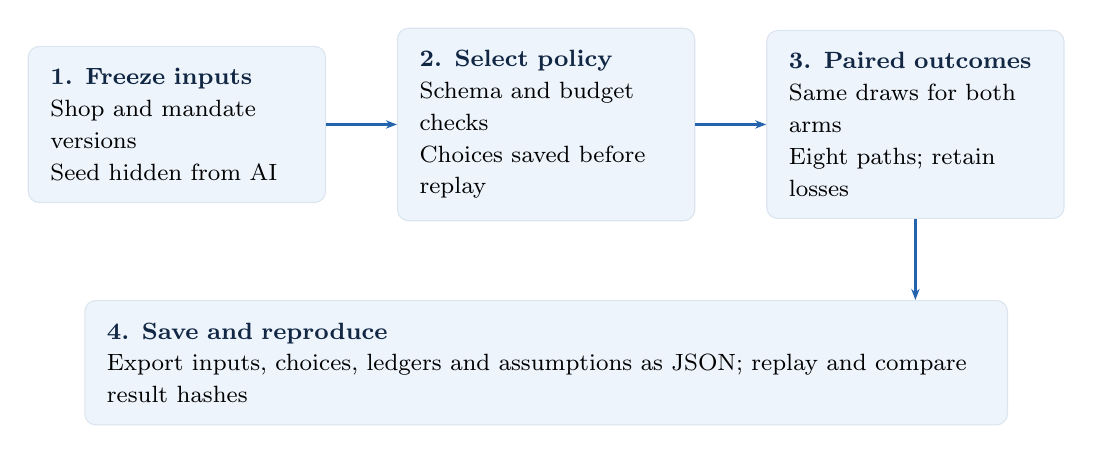
\begin{tikzpicture}[node distance=9mm]
  \node[docbox] (inputs) {\textcolor{Navy}{\bfseries 1. Freeze inputs}\\Shop and mandate versions\\Seed hidden from AI};
  \node[docbox,right=of inputs] (choices) {\textcolor{Navy}{\bfseries 2. Select policy}\\Schema and budget checks\\Choices saved before replay};
  \node[docbox,right=of choices] (outcomes) {\textcolor{Navy}{\bfseries 3. Paired outcomes}\\Same draws for both arms\\Eight paths; retain losses};
  \node[docbox,below=10mm of choices,text width=0.92\linewidth] (export) {\textcolor{Navy}{\bfseries 4. Save and reproduce}\\Export inputs, choices, ledgers and assumptions as JSON; replay and compare result hashes};
  \draw[flow] (inputs)--(choices);\draw[flow] (choices)--(outcomes);\draw[flow] (outcomes.south)--(outcomes.south |- export.north);
\end{tikzpicture}\end{center}}
